\documentclass{standalone}
\usepackage{tikz}
\usetikzlibrary{patterns, positioning}

\begin{document}
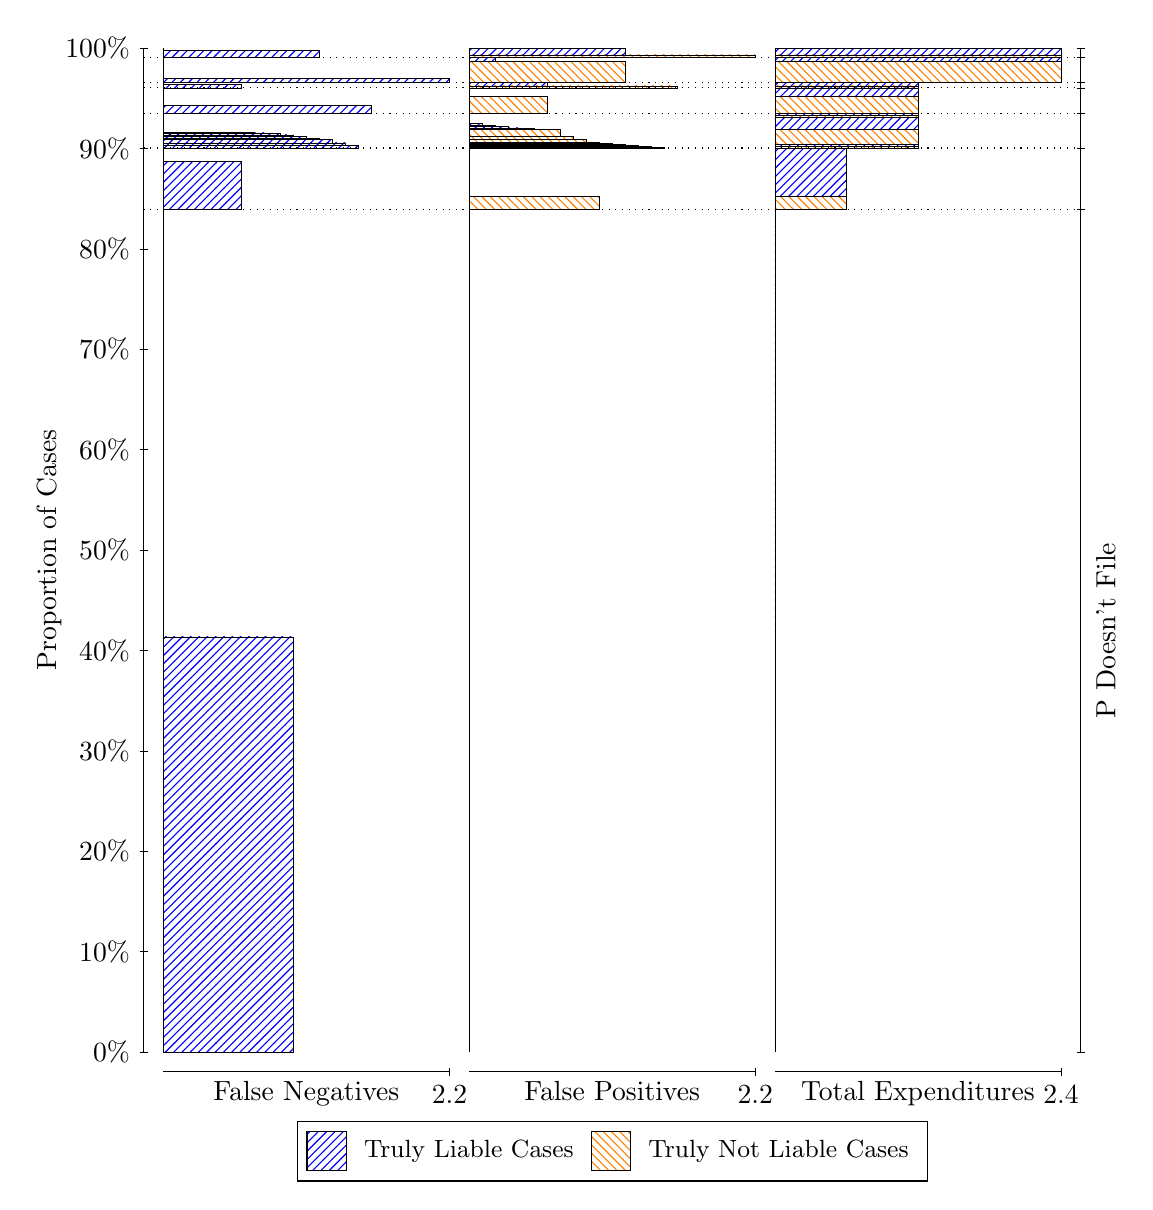
\begin{tikzpicture}
\draw[black, very thin] (1.5,1.75) -- (1.5,14.5);
\node[rotate=90, anchor=center] at (0.3, 8.125) {Proportion of Cases};
\draw[black, very thin] (1.45,1.75) -- (1.55,1.75);
\node[anchor=east] at (1.45, 1.75) {0\%};
\draw[black, very thin] (1.45,3.025) -- (1.55,3.025);
\node[anchor=east] at (1.45, 3.025) {10\%};
\draw[black, very thin] (1.45,4.3) -- (1.55,4.3);
\node[anchor=east] at (1.45, 4.3) {20\%};
\draw[black, very thin] (1.45,5.575) -- (1.55,5.575);
\node[anchor=east] at (1.45, 5.575) {30\%};
\draw[black, very thin] (1.45,6.85) -- (1.55,6.85);
\node[anchor=east] at (1.45, 6.85) {40\%};
\draw[black, very thin] (1.45,8.125) -- (1.55,8.125);
\node[anchor=east] at (1.45, 8.125) {50\%};
\draw[black, very thin] (1.45,9.4) -- (1.55,9.4);
\node[anchor=east] at (1.45, 9.4) {60\%};
\draw[black, very thin] (1.45,10.675) -- (1.55,10.675);
\node[anchor=east] at (1.45, 10.675) {70\%};
\draw[black, very thin] (1.45,11.95) -- (1.55,11.95);
\node[anchor=east] at (1.45, 11.95) {80\%};
\draw[black, very thin] (1.45,13.225) -- (1.55,13.225);
\node[anchor=east] at (1.45, 13.225) {90\%};
\draw[black, very thin] (1.45,14.5) -- (1.55,14.5);
\node[anchor=east] at (1.45, 14.5) {100\%};

\draw[black, very thin] (13.4,1.75) -- (13.4,14.5);
\draw[black, very thin] (13.35,1.75) -- (13.45,1.75);
\node[anchor=west] at (13.35, 1.75) {};
\draw[black, very thin] (13.35,12.447) -- (13.45,12.447);
\node[anchor=west] at (13.35, 12.447) {};
\draw[black, very thin] (13.35,13.23) -- (13.45,13.23);
\node[anchor=west] at (13.35, 13.23) {};
\draw[black, very thin] (13.35,13.669) -- (13.45,13.669);
\node[anchor=west] at (13.35, 13.669) {};
\draw[black, very thin] (13.35,13.995) -- (13.45,13.995);
\node[anchor=west] at (13.35, 13.995) {};
\draw[black, very thin] (13.35,14.065) -- (13.45,14.065);
\node[anchor=west] at (13.35, 14.065) {};
\draw[black, very thin] (13.35,14.379) -- (13.45,14.379);
\node[anchor=west] at (13.35, 14.379) {};
\draw[black, very thin] (13.35,14.5) -- (13.45,14.5);
\node[anchor=west] at (13.35, 14.5) {};

\draw[black, very thin, pattern color=blue, pattern=north east lines] (1.75,1.75) rectangle (3.4015,7.0227);
\draw[black, very thin, pattern color=orange, pattern=north west lines] (1.75,7.0227) rectangle (1.75,12.447);
\draw[black, very thin, pattern color=blue, pattern=north east lines] (1.75,12.447) rectangle (2.7409,13.059);
\draw[black, very thin, pattern color=orange, pattern=north west lines] (1.75,13.059) rectangle (1.75,13.23);
\draw[black, very thin, pattern color=blue, pattern=north east lines] (1.75,13.23) rectangle (4.2273,13.266);
\draw[black, very thin, pattern color=blue, pattern=north east lines] (1.75,13.266) rectangle (4.0621,13.295);
\draw[black, very thin, pattern color=blue, pattern=north east lines] (1.75,13.295) rectangle (3.897,13.337);
\draw[black, very thin, pattern color=blue, pattern=north east lines] (1.75,13.337) rectangle (3.7318,13.354);
\draw[black, very thin, pattern color=blue, pattern=north east lines] (1.75,13.354) rectangle (3.5667,13.379);
\draw[black, very thin, pattern color=blue, pattern=north east lines] (1.75,13.379) rectangle (3.4015,13.396);
\draw[black, very thin, pattern color=blue, pattern=north east lines] (1.75,13.396) rectangle (3.2364,13.412);
\draw[black, very thin, pattern color=blue, pattern=north east lines] (1.75,13.412) rectangle (3.0712,13.422);
\draw[black, very thin, pattern color=blue, pattern=north east lines] (1.75,13.422) rectangle (2.9061,13.431);
\draw[black, very thin, pattern color=orange, pattern=north west lines] (1.75,13.431) rectangle (1.75,13.669);
\draw[black, very thin, pattern color=blue, pattern=north east lines] (1.75,13.669) rectangle (4.3924,13.774);
\draw[black, very thin, pattern color=orange, pattern=north west lines] (1.75,13.774) rectangle (1.75,13.995);
\draw[black, very thin, pattern color=blue, pattern=north east lines] (1.75,13.995) rectangle (2.7409,14.04);
\draw[black, very thin, pattern color=orange, pattern=north west lines] (1.75,14.04) rectangle (1.75,14.065);
\draw[black, very thin, pattern color=blue, pattern=north east lines] (1.75,14.065) rectangle (5.3833,14.115);
\draw[black, very thin, pattern color=orange, pattern=north west lines] (1.75,14.115) rectangle (1.75,14.379);
\draw[black, very thin, pattern color=blue, pattern=north east lines] (1.75,14.379) rectangle (3.7318,14.466);
\draw[black, very thin, pattern color=orange, pattern=north west lines] (1.75,14.466) rectangle (1.75,14.5);
\draw[black, very thin, pattern color=orange, pattern=north west lines] (5.6333,1.75) rectangle (5.6333,7.1739);
\draw[black, very thin, pattern color=blue, pattern=north east lines] (5.6333,7.1739) rectangle (5.6333,12.447);
\draw[black, very thin, pattern color=orange, pattern=north west lines] (5.6333,12.447) rectangle (7.2848,12.618);
\draw[black, very thin, pattern color=blue, pattern=north east lines] (5.6333,12.618) rectangle (5.6333,13.23);
\draw[black, very thin, pattern color=orange, pattern=north west lines] (5.6333,13.23) rectangle (8.1106,13.238);
\draw[black, very thin, pattern color=orange, pattern=north west lines] (5.6333,13.238) rectangle (7.9455,13.246);
\draw[black, very thin, pattern color=orange, pattern=north west lines] (5.6333,13.246) rectangle (7.7803,13.26);
\draw[black, very thin, pattern color=orange, pattern=north west lines] (5.6333,13.26) rectangle (7.6152,13.273);
\draw[black, very thin, pattern color=orange, pattern=north west lines] (5.6333,13.273) rectangle (7.45,13.293);
\draw[black, very thin, pattern color=orange, pattern=north west lines] (5.6333,13.293) rectangle (7.2848,13.306);
\draw[black, very thin, pattern color=orange, pattern=north west lines] (5.6333,13.306) rectangle (7.1197,13.344);
\draw[black, very thin, pattern color=orange, pattern=north west lines] (5.6333,13.344) rectangle (6.9545,13.373);
\draw[black, very thin, pattern color=orange, pattern=north west lines] (5.6333,13.373) rectangle (6.7894,13.468);
\draw[black, very thin, pattern color=blue, pattern=north east lines] (5.6333,13.468) rectangle (6.4591,13.478);
\draw[black, very thin, pattern color=blue, pattern=north east lines] (5.6333,13.478) rectangle (6.2939,13.487);
\draw[black, very thin, pattern color=blue, pattern=north east lines] (5.6333,13.487) rectangle (6.1288,13.504);
\draw[black, very thin, pattern color=blue, pattern=north east lines] (5.6333,13.504) rectangle (5.9636,13.52);
\draw[black, very thin, pattern color=blue, pattern=north east lines] (5.6333,13.52) rectangle (5.7985,13.545);
\draw[black, very thin, pattern color=blue, pattern=north east lines] (5.6333,13.545) rectangle (5.6333,13.669);
\draw[black, very thin, pattern color=orange, pattern=north west lines] (5.6333,13.669) rectangle (6.6242,13.889);
\draw[black, very thin, pattern color=blue, pattern=north east lines] (5.6333,13.889) rectangle (5.6333,13.995);
\draw[black, very thin, pattern color=orange, pattern=north west lines] (5.6333,13.995) rectangle (8.2758,14.019);
\draw[black, very thin, pattern color=blue, pattern=north east lines] (5.6333,14.019) rectangle (6.6242,14.065);
\draw[black, very thin, pattern color=orange, pattern=north west lines] (5.6333,14.065) rectangle (7.6152,14.329);
\draw[black, very thin, pattern color=blue, pattern=north east lines] (5.6333,14.329) rectangle (5.9636,14.379);
\draw[black, very thin, pattern color=orange, pattern=north west lines] (5.6333,14.379) rectangle (9.2667,14.413);
\draw[black, very thin, pattern color=blue, pattern=north east lines] (5.6333,14.413) rectangle (7.6152,14.5);
\draw[black, very thin, pattern color=orange, pattern=north west lines] (9.5167,1.75) rectangle (9.5167,7.1739);
\draw[black, very thin, pattern color=blue, pattern=north east lines] (9.5167,7.1739) rectangle (9.5167,12.447);
\draw[black, very thin, pattern color=orange, pattern=north west lines] (9.5167,12.447) rectangle (10.425,12.618);
\draw[black, very thin, pattern color=blue, pattern=north east lines] (9.5167,12.618) rectangle (10.425,13.23);
\draw[black, very thin, pattern color=orange, pattern=north west lines] (9.5167,13.23) rectangle (11.333,13.25);
\draw[black, very thin, pattern color=blue, pattern=north east lines] (9.5167,13.25) rectangle (11.333,13.275);
\draw[black, very thin, pattern color=orange, pattern=north west lines] (9.5167,13.275) rectangle (11.333,13.471);
\draw[black, very thin, pattern color=blue, pattern=north east lines] (9.5167,13.471) rectangle (11.333,13.621);
\draw[black, very thin, pattern color=orange, pattern=north west lines] (9.5167,13.621) rectangle (11.333,13.643);
\draw[black, very thin, pattern color=blue, pattern=north east lines] (9.5167,13.643) rectangle (11.333,13.669);
\draw[black, very thin, pattern color=orange, pattern=north west lines] (9.5167,13.669) rectangle (11.333,13.889);
\draw[black, very thin, pattern color=blue, pattern=north east lines] (9.5167,13.889) rectangle (11.333,13.995);
\draw[black, very thin, pattern color=orange, pattern=north west lines] (9.5167,13.995) rectangle (11.333,14.019);
\draw[black, very thin, pattern color=blue, pattern=north east lines] (9.5167,14.019) rectangle (11.333,14.065);
\draw[black, very thin, pattern color=orange, pattern=north west lines] (9.5167,14.065) rectangle (13.15,14.329);
\draw[black, very thin, pattern color=blue, pattern=north east lines] (9.5167,14.329) rectangle (13.15,14.379);
\draw[black, very thin, pattern color=orange, pattern=north west lines] (9.5167,14.379) rectangle (13.15,14.413);
\draw[black, very thin, pattern color=blue, pattern=north east lines] (9.5167,14.413) rectangle (13.15,14.5);
\draw[black, dotted] (1.5,12.447) -- (13.4,12.447);
\draw[black, dotted] (1.5,13.23) -- (13.4,13.23);
\draw[black, dotted] (1.5,13.669) -- (13.4,13.669);
\draw[black, dotted] (1.5,13.995) -- (13.4,13.995);
\draw[black, dotted] (1.5,14.065) -- (13.4,14.065);
\draw[black, dotted] (1.5,14.379) -- (13.4,14.379);
\draw[black, very thin] (1.75,1.5) -- (5.3833,1.5);
\node[anchor=north] at (3.5667, 1.5) {False Negatives};
\draw[black, very thin] (5.3833,1.45) -- (5.3833,1.55);
\node[anchor=north] at (5.3833, 1.45) {2.2};

\draw[black, very thin] (5.6333,1.5) -- (9.2667,1.5);
\node[anchor=north] at (7.45, 1.5) {False Positives};
\draw[black, very thin] (9.2667,1.45) -- (9.2667,1.55);
\node[anchor=north] at (9.2667, 1.45) {2.2};

\draw[black, very thin] (9.5167,1.5) -- (13.15,1.5);
\node[anchor=north] at (11.333, 1.5) {Total Expenditures};
\draw[black, very thin] (13.15,1.45) -- (13.15,1.55);
\node[anchor=north] at (13.15, 1.45) {2.4};

\node[black, centered, rotate=90] at (13.72, 7.0983) {P Doesn't File};







\draw (7.449999999999999,1.5) node[draw=none] (baseCoordinate) {};
\begin{scope}[align=center]
        \matrix[scale=0.5, draw=black, below=0.5cm of baseCoordinate, nodes={draw}, column sep=0.1cm]{
            \node[rectangle, draw, minimum width=0.5cm, minimum height=0.5cm, pattern=north east lines, pattern color=blue] {}; &
            \node[draw=none, font=\small] (B) {Truly Liable Cases}; &
            \node[rectangle, draw, minimum width=0.5cm, minimum height=0.5cm, pattern=north west lines, pattern color=orange] {}; &
            \node[draw=none, font=\small] (B) {Truly Not Liable Cases}; \\
            };
\end{scope}

\end{tikzpicture}
\end{document}